\documentclass[11pt]{book}
\usepackage{palatino}
\usepackage{amsfonts,amsmath,amssymb}
% \usepackage{graphicx}


\ifx\pdftexversion\undefined
    \usepackage[dvips]{graphicx}
\else
    \usepackage[pdftex]{graphicx}
    \usepackage{epstopdf}
    \epstopdfsetup{suffix=}
\fi


\begin{document}

%%%%%%%%%%%%%%%%%%%%%%%%%%%%%%%%%%%%%%%%
% Problem Set 5
%%%%%%%%%%%%%%%%%%%%%%%%%%%%%%%%%%%%%%%%

\pagestyle{empty}
{\noindent\bf Spring 2021 \hfill Firstname M.~Lastname}
\vskip 16pt
\centerline{\bf University of Central Florida}
\centerline{\bf College of Business}
\vskip 16pt
\centerline{\bf QMB 6911}
\centerline{\bf Capstone Project in Business Analytics}
\vskip 10pt
\centerline{\bf Solutions:  Problem Set \#5}
\vskip 32pt
\noindent


\section*{Scatterplot Matrices}


\subsection*{Scatterplots of Numeric Variables}

Figure \ref{fig:slpom_num_only} depicts a matrix of scatterplots
of the numeric variables in the dataset.

\begin{figure}[h!]
  \centering
  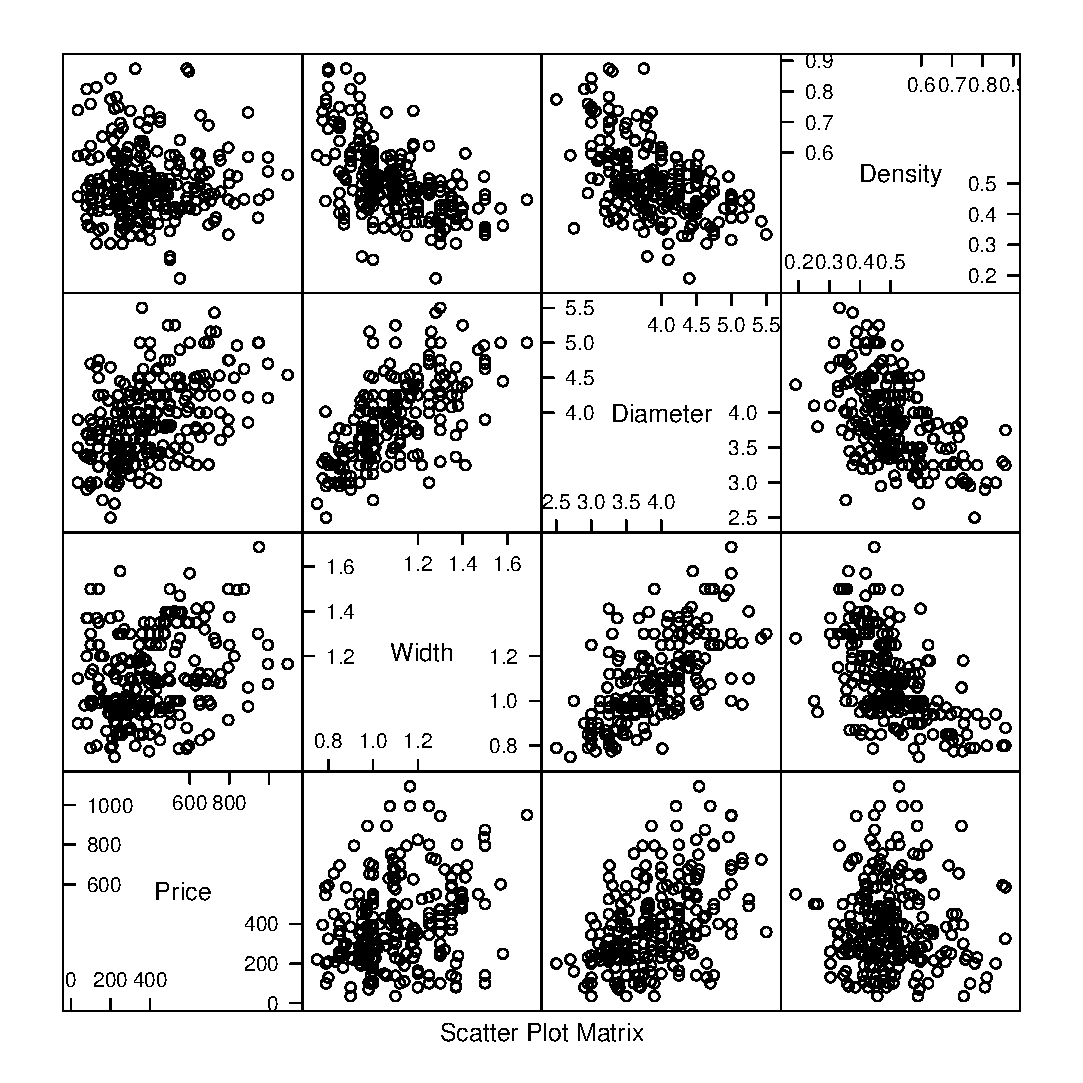
\includegraphics[scale = 0.5, keepaspectratio=true]{../Figures/slpom_num_only}
  \caption{Scatterplots of Numeric Variables} \label{fig:slpom_num_only}
\end{figure}


\pagebreak
\subsection*{Scatterplots with Categorical Variables}

Figure \ref{fig:slpom_with_cat} depicts a matrix of scatterplots
of with categorical variables in the dataset.

\begin{figure}[h!]
  \centering
  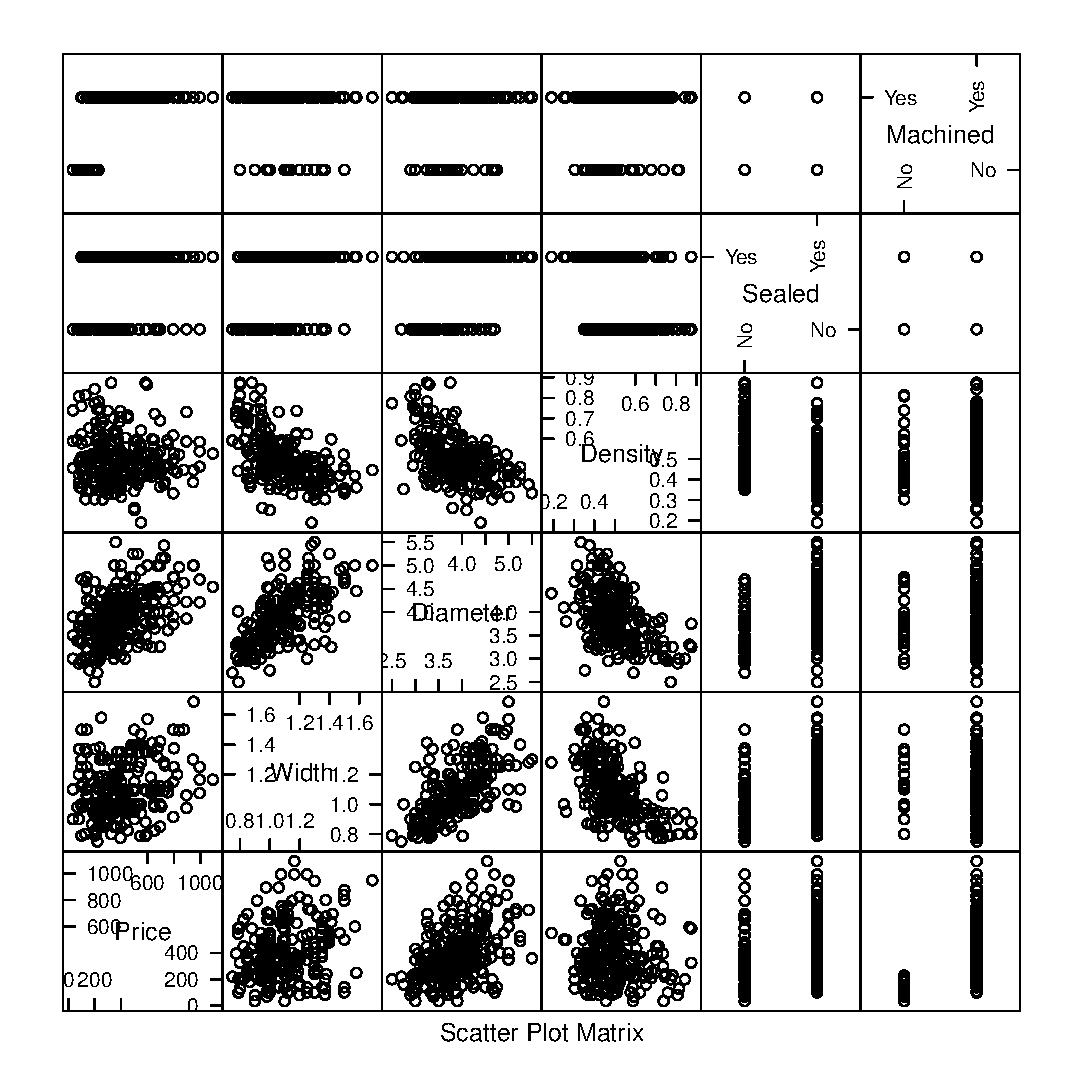
\includegraphics[scale = 0.5, keepaspectratio=true]{../Figures/slpom_with_cat}
  \caption{Scatterplots with Categorical Variables} \label{fig:slpom_with_cat}
\end{figure}


\pagebreak


Figure \ref{fig:slpom_with_sealed_mach.eps} depicts a matrix of scatterplots
with a categorical variable for the design combinations of the fly reels:
a fly reel is either sealed or unsealed and either machined or cast.

\begin{figure}[h!]
  \centering
  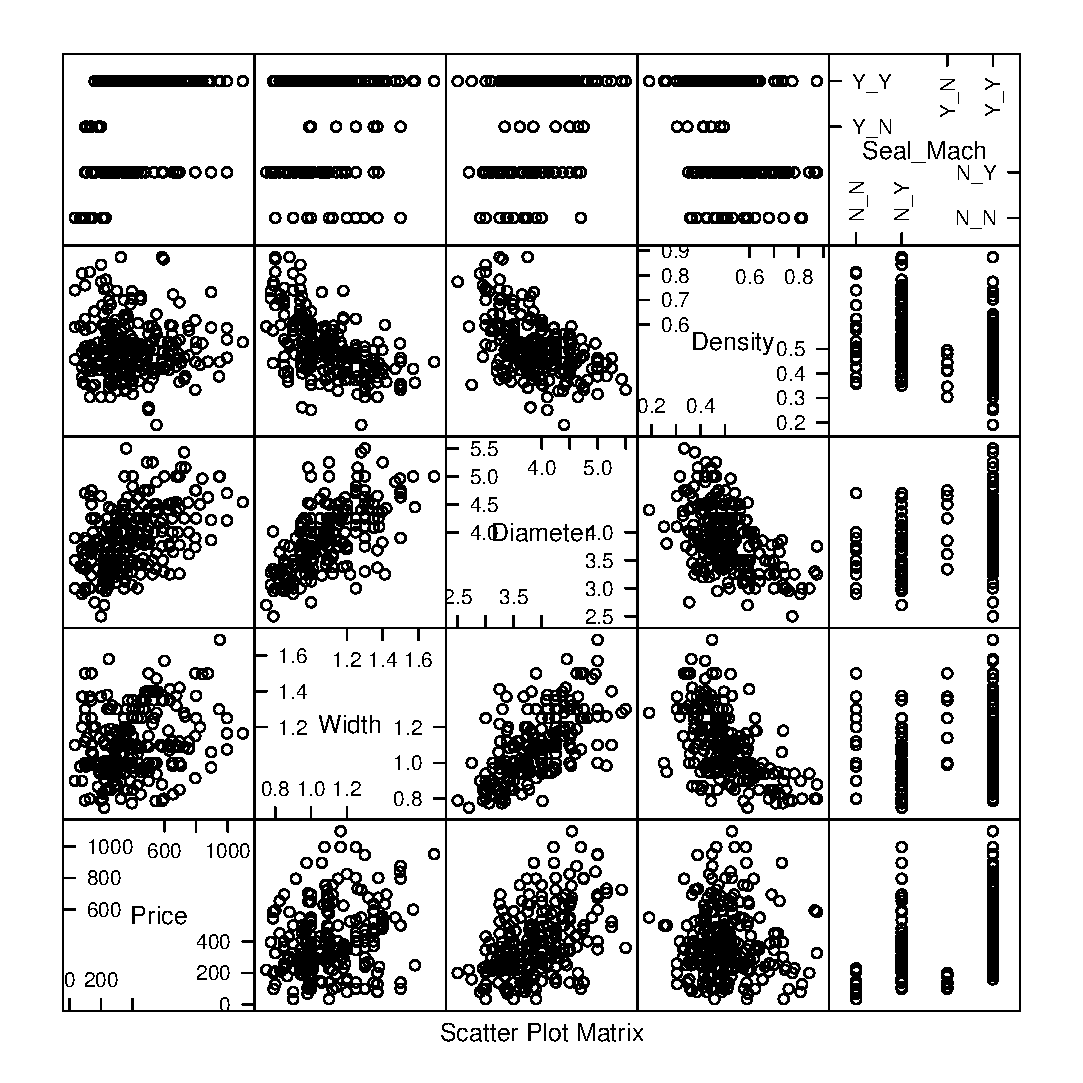
\includegraphics[scale = 0.5, keepaspectratio=true]{../Figures/slpom_with_sealed_mach.eps}
  \caption{Scatterplots of Numeric Variables} \label{fig:slpom_with_sealed_mach.eps}
\end{figure}



\pagebreak
\subsection*{Scatterplots by Country of Manufacture}

Figure \ref{fig:slpom_by_country} depicts a matrix of scatterplots
of the variables in the dataset
with the points color-coded by country of manufacture.

\begin{figure}[h!]
  \centering
  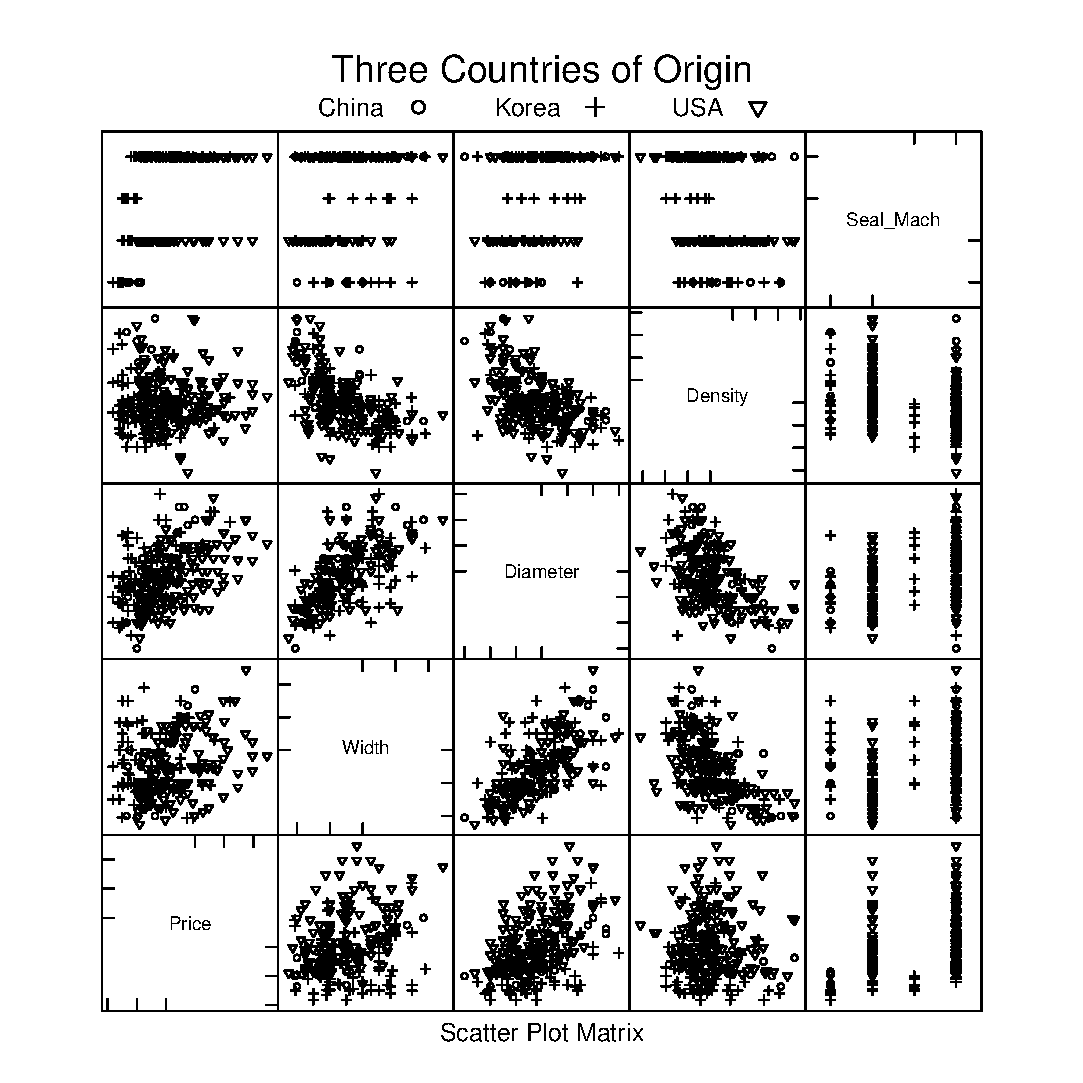
\includegraphics[scale = 0.5, keepaspectratio=true]{../Figures/slpom_by_country}
  \caption{Scatterplots by Country of Manufacture} \label{fig:slpom_by_country}
\end{figure}




%%%%%%%%%%%%%%%%%%%%%%%%%%%%%%%%%%%%%%%%
\end{document}
%%%%%%%%%%%%%%%%%%%%%%%%%%%%%%%%%%%%%%%%
